\section{Experiment}
Our setup consists of a glass bulb with a pre-installed pressure sensor, connected to a voltmeter, a pump for evacuating the bulb and a balloon, which is again connected to a bottle filled with helium as shown in figure \ref{fig::shema}. 

\begin{figure}[h]
	\centering
	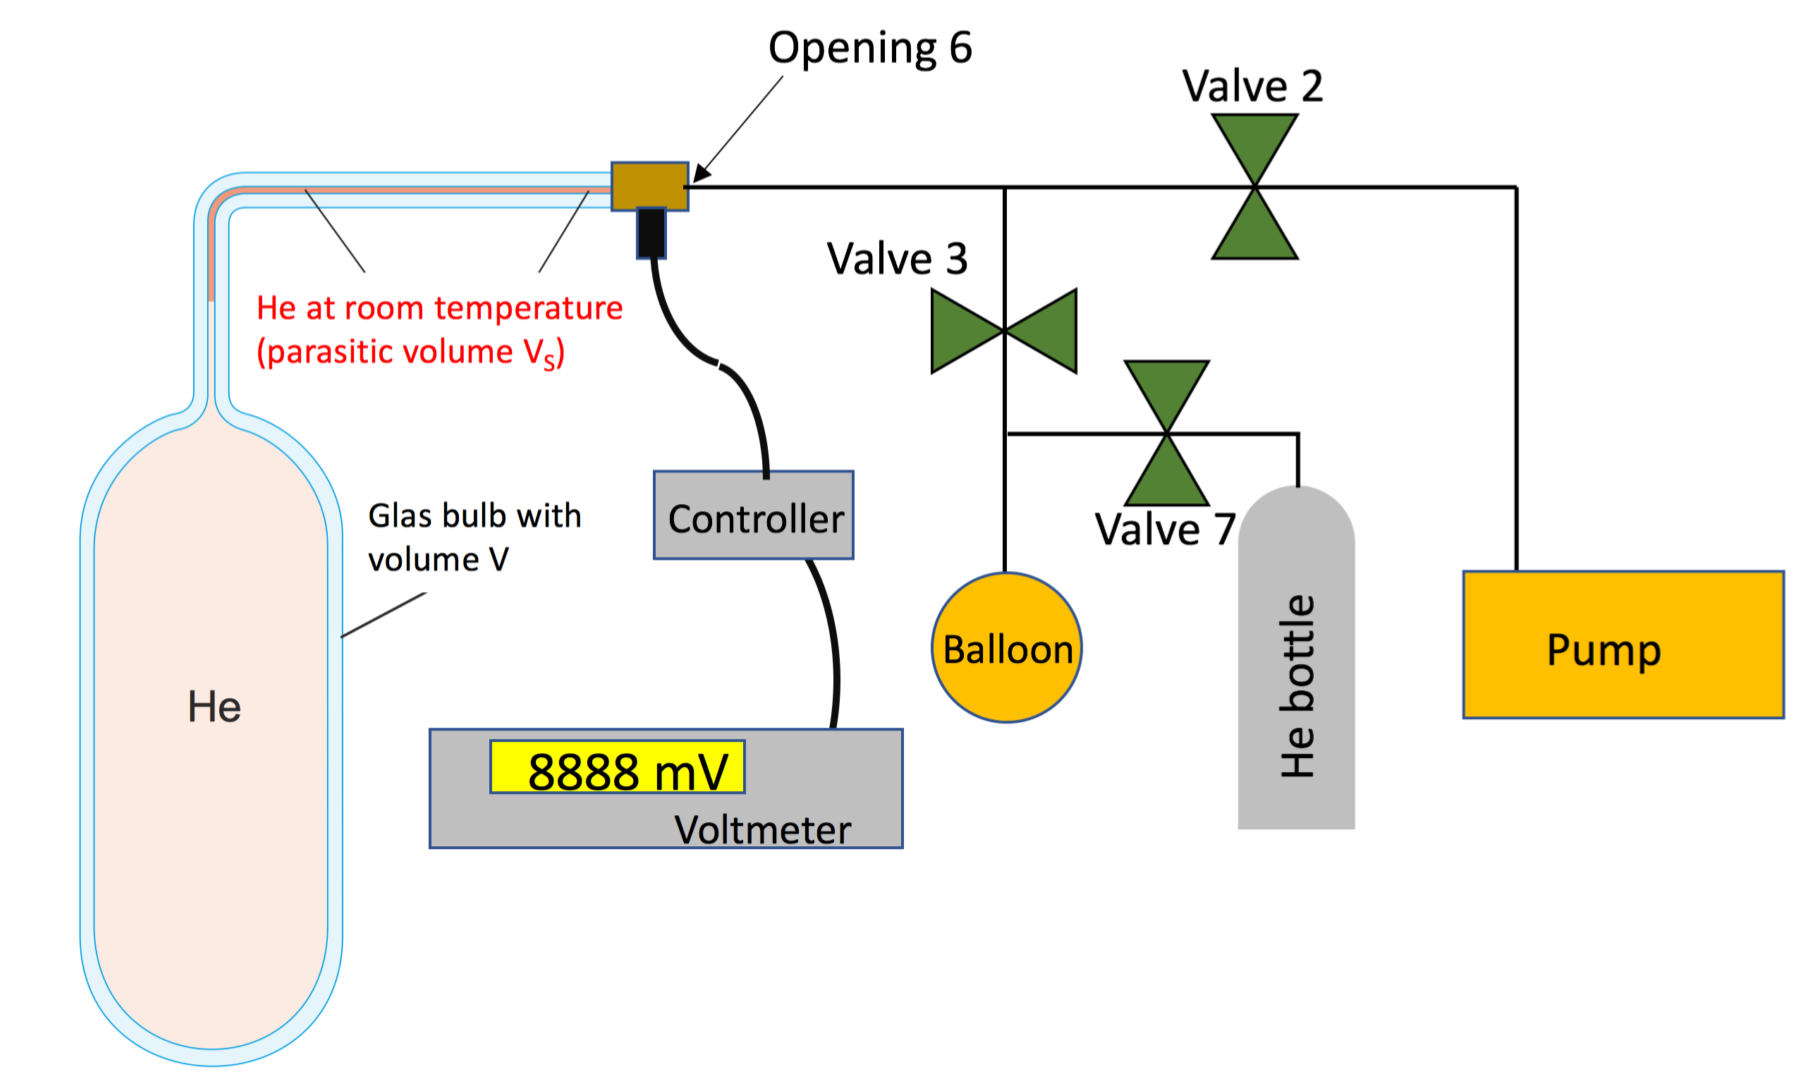
\includegraphics[width=0.7\textwidth]{sections/images/schematic.png}
	\caption{Schematic taken from the experiment manual\label{fig::shema}}
\end{figure}

\paragraph{1. Step}
Our first task is to calibrate the pressure sensor as it outputs just voltage, not pressure directly. For that we need to measure voltages of two known pressures, in our case the air pressure $p_L$ in the lab and the one of near vacuum $p_t$. To evaluate the air pressure there is a mercury barometer available in the lab. First we get the signal $U_L$ from exposing the sensor to air pressure. After that, we evacuate the bulb with the pump and get $U_t$, the voltage at near vacuum (the pump should be able to produce a pressure significantly below \SI{0.2}{\milli\bar}). From those two measurements we can evaluate the slope $C$ and the offset $p_0$ of the so called characteristic curve of the sensor. Now we can convert the measured voltage to a pressure value with the following formula.

\begin{align}
	p(U) = p_0 + CU
	\label{eq::convert}
\end{align}

\paragraph{2. Step}
\label{para:2}
The next step is the experimental part. As said before we want to measure the pressure of a given amount of gas in a constant volume at two different known temperatures. 

To begin we need to fill the glass bulb with helium. 
Since we want no air remaining in the bulb, we evacuate it first, fill it with helium, and then repeat this process once. 
Filling the bulb with too much pressure should be avoided.
Thus we first fill a balloon with helium and later fill the glass bulb from this balloon. 
To have enough helium in the balloon, the size should be around the size of a football. 
From there, we fill the glass bulb with helium and not from the helium bottle directly. 
We remove the hose at opening 6 in figure \ref{fig::shema} before exposing the bulb to heat. 
Because the pressure in the bulb will increase, air will not get into the bulb. 


We place a water cooker under the bulb with a container, so the bulb will be exposed to the vapour as good as possible. 
After the voltage has settled we close opening 6 from figure \ref{fig::shema}, read the signal of the sensor which is our $U_k$ and convert it to pressure value $p_k$ using equation \ref{eq::convert}. 
We can determine the assumed boiling temperature of water with our measured air pressure and a conversion table supplied in the lab. 


Next we place the bulb in a container filled with ice and water to have a temperature as close to zero degrees Celsius as possible. 
Again, after the voltage signal has settled, we can read our pressure value $U_e$ and calculate $p_e$ using the equation \ref{eq::convert}.


With these two values and the knowledge from the ideal gas equation \ref{eq::gas}, the absolute zero point is calculated.
The exact calculations can be seen in the section data analysis.

\paragraph{3. Step}
In the last part of the experiment, we want to use our setup as a thermometer and measure the temperature of liquid nitrogen. 
For that we completely submerge the sealed glass bulb as it is, in a container of liquid nitrogen, read the voltage $U_n$ corresponding to the pressure value and calculate $p_n$.


